\chapter{Método de trabajo}
\label{chap:metodo}

\drop{E}{}sta sección está centrada en detallar y justificar la metodología usada durante la elaboración del proyecto, de tal forma que se exponga al lector cómo ha sido llevado a cabo el desarrollo a nivel organizativo. Conjuntamente, se especifican los medios hardware y software que han sido utilizados a lo largo de todo el \acs{TFG}.

\section{Metodología}
\label{sec:metodologia}

Para la elección de la metodología de trabajo se debe escoger una que se ajuste a las condiciones del proyecto, es decir, que satisfaga la dinámica de trabajo que se desea seguir. Por lo cual es primordial que la metodología elegida divida el \textbf{desarrollo en hitos} que son potencialmente entregables y que no contienen errores. Igualmente, se debe tener en consideración el contexto donde se desarrolla el sistema. En este proyecto, al tiempo que se realiza el desarrollo del sistema es plausible que aparezcan complicaciones, por lo que es preciso que la metodología sea flexible, en otras palabras, que sea posible corregir las tareas con respecto a los inconvenientes que aparecerán durante el progreso del proyecto, conservando como línea de referencia los objetivos precisados (Referenciar Capitulo de objetivos).

En consecuencia, se excluyen las metodologías de desarrollo tradicionales, basadas en una planificación inicial que permanece intacta de principio a fin. Se decide escoger una \textbf{metodología de desarrollo ágil} cuyo principal objetivo es desarrollar proyectos de forma \textbf{iterativa e incremental}, en la que puedan definirse objetivos en cada iteración. La preferencia sobre una metodología ágil posibilita la entrega, en un periodo de tiempo reducido, de un proyecto funcional y que el usuario pueda evaluar. Entre las metodologías de desarrollo ágil existe un amplio abanico donde elegir: Programación Extrema, Desarrollo Adaptativo de Software, \textbf{Scrum}, etcétera. De ellas, Scrum es la que mejor se ajusta a las exigencias del proyecto.

\subsection{Manifiesto ágil}
\label{sec:manifiestoagil}

Para comprender mejor la filosofía tras las metodologías ágiles, seguidamente se cita el \textbf{Manifiesto Ágil} \footnote{\url{http://www.agilemanifesto.org/iso/es/}} y sus cuatro valores:

«Estamos descubriendo formas mejores de desarrollar software tanto por nuestra propia experiencia como ayudando a terceros. A través de este trabajo hemos aprendido a valorar:

\begin{itemize}
\item \textbf{Individuos e interacciones} sobre \textbf{procesos y herramientas}.
\item \textbf{Software funcionando} sobre \textbf{documentación extensiva}.
\item \textbf{Colaboración con el cliente} sobre \textbf{negociación contractual}.
\item \textbf{Respuesta ante el cambio} sobre \textbf{seguir un plan}.
\end{itemize}

Esto es, aunque valoramos los elementos de la derecha, valoramos más los de la izquierda». De estos cuatro valores, se desarrollaron doce principios para el Manifiesto Ágil \footnote{\url{http://agilemanifesto.org/iso/es/principles.html}}, que son:

\begin{itemize}
\item La mayor prioridad es \textbf{satisfacer al cliente} mediante la entrega temprana y continua de software con valor.
\item \textbf{Aceptar} que los \textbf{requisitos cambien}, incluso en etapas tardías del desarrollo. Los procesos Ágiles aprovechan el cambio para proporcionar ventaja competitiva al cliente.
\item Se \textbf{entrega} software funcional \textbf{frecuentemente}, entre dos semanas y dos meses, con preferencia al periodo de tiempo más corto posible.
\item Los \textbf{responsables} de negocio, en este caso David Vallejo como director del proyecto, y los \textbf{desarrolladores trabajan juntos} de forma cotidiana durante todo el proyecto.
\item Los proyectos se desarrollan en torno a \textbf{individuos motivados}. Hay que darles el entorno y el apoyo que necesitan, y confiarles la ejecución del trabajo.
\item El método más eficiente y efectivo de \textbf{comunicar información} al equipo de desarrollo y entre sus miembros es la conversación \textbf{cara a cara}. 
\item El \textbf{software funcionando} es la \textbf{medida principal de progreso}.
\item Los procesos Ágiles promueven el \textbf{desarrollo sostenible}. Los promotores, desarrolladores y usuarios debemos ser capaces de mantener un ritmo constante de forma indefinida.
\item La \textbf{atención continua} a la excelencia técnica y al buen diseño \textbf{mejora la Agilidad}.
\item La \textbf{simplicidad}, o el arte de maximizar la cantidad de trabajo no realizado, \textbf{es esencial}.
\item Las mejores arquitecturas, requisitos y diseños emergen de \textbf{equipos auto-organizados}.
\item A intervalos regulares \textbf{el equipo reflexiona sobre cómo ser más efectivo} para a continuación ajustar y perfeccionar su comportamiento en consecuencia. 
\end{itemize}

\subsection{Scrum}
\label{sec:scrum}

La metodología de trabajo \textbf{Scrum} «requiere que los equipos completen algún tipo de producto potencialmente liberable al final de cada iteración. Estas iteraciones están diseñadas para ser cortas y de duración fija. Este enfoque en entregar código funcional cada poco tiempo significa que los equipos Scrum no tienen tiempo para teorías. No persiguen dibujar el modelo UML perfecto en una herramienta CASE, escribir el documento de requisitos perfecto o escribir código que se adapte a todos los cambios futuros imaginables. En vez de eso, los equipos Scrum se enfocan en que las cosas se hagan. Estos equipos aceptan que puede que se equivoquen por el camino, pero también son conscientes de que la mejor manera de encontrar dichos errores es dejar de pensar en el software a un nivel teórico de análisis y diseño y sumergirse en él, ensuciarse las manos y comenzar a construir el producto» \cite{scrum}.

Por consiguiente, se puede definir Scrum como un framework, dentro del cual se pueden emplear varias técnicas y procesos, para el manejo de proyectos que tienen como fin el desarrollo de productos complejos. Scrum tiene sus orígenes en los campos del manejo del conocimiento, los sistemas adaptativos complejos y la teoría de control empírico de procesos. Ha sido influenciado también de patrones observados durante el desarrollo de software y la Teoría de las Limitaciones.

Una fortaleza clave de Scrum radica en el uso de equipos interfuncionales, auto-organizados, y empoderados que dividen su trabajo en ciclos de trabajo cortos y concentrados llamados Sprints.

El ciclo de Scrum (ver Figura~\ref{fig:scrum}). comienza con una reunión, durante la cual se crea la visión del proyecto. Después, el propietario del producto desarrolla una Lista priorizada que contiene una lista de requerimientos del negocio por orden de importancia. 
Cada sprint comienza con una reunión de planificación del sprint. Un sprint suele durar entre una y seis semanas durante las cuales el equipo trabaja en la creación de entregables que incrementen la funcionalidad del producto. Durante el sprint, se llevan cabo reuniones muy breves y concretas en las que los miembros del equipo discuten progresos diarios. A medida que concluye el sprint, se lleva a cabo una reunión de planificación del sprint en la cual se proporciona una demostración de los entregables al propietario del producto y a los socios relevantes. El propietario del producto acepta los entregables sólo si cumplen con los criterios de aceptación predefinidos.

\begin{figure}[!h]
\begin{center}
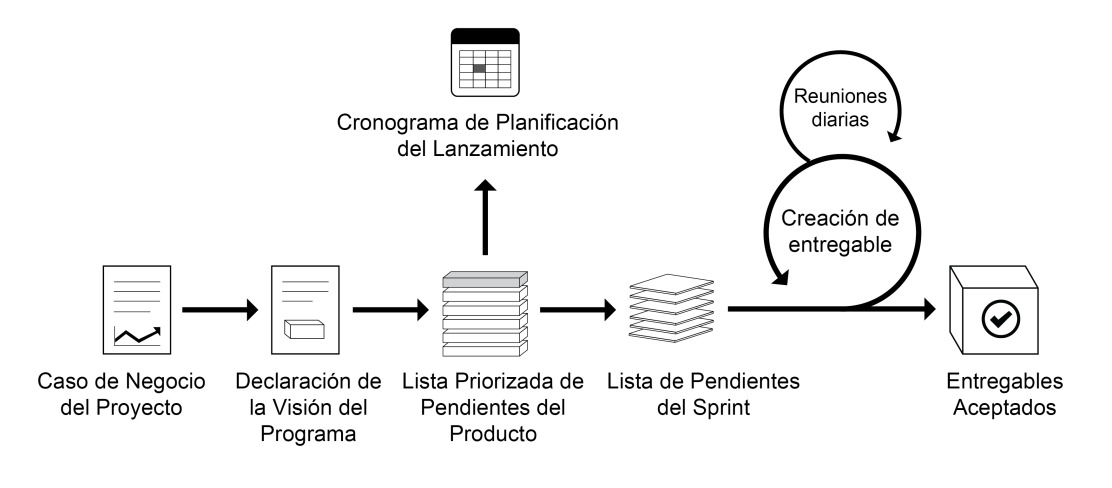
\includegraphics[width=0.8\textwidth]{/scrum.jpg}
\caption[Flujo de Scrum para un Sprint]{Flujo de Scrum para un Sprint}
\label{fig:scrum}
\end{center}
\end{figure}


% Local Variables:
% coding: utf-8
% mode: latex
% mode: flyspell
% ispell-local-dictionary: "castellano8"
% End:
